%\title{יומן פיתוח פרוייקט}

\documentclass{report}
\usepackage[utf8x]{inputenc}
\usepackage[english,hebrew]{babel}
\usepackage{datetime}
\usepackage{ragged2e}
\usepackage{minted}
\usepackage{xcolor} % to access the named colour LightGray
\usepackage{listings}
\usepackage{graphicx}
\definecolor{LightGray}{gray}{0.9}
\selectlanguage{hebrew}
\usepackage[top=2cm,bottom=2cm,left=2.5cm,right=2cm]{geometry}
\title{יומן פיתוח פרוייקט}
\author{דניס שרבקוב}
\newdate{Initialcreation}{01}{09}{2023}
\newdate{firstchange}{14}{02}{2024}
\newdate{change2}{24}{02}{2024}
\graphicspath{{./images/}}

\date{\displaydate{Initialcreation}}
\begin{document}
\maketitle

\tableofcontents

\newpage
\chapter{מבוא}
\section{הפרוייקט}
מטרת הפרוייקט היא לספק אתר שישמש ככלי עזר לקבלת החלטות לגבי קניות של מוצרי הבית היום-יומיים האתר יכיל מגוון רחב של מידע לגבי שלל מוצרים ויספק אלטרנטיבות קניה "ירוקות" למשתמש על מנת שיוכל לבצע קניות באופן ששומר על הסביבה ברמה המירבית
\subsection{כיצד עובד האתר?}
האתר ימלא את תפקידו בעזרת שימוש במערכת דמויית \L{Wiki} שתאפשר למשתמשים להזין מידע לאתר בכוחות עצמם לגבי מגוון מוצרים
\newpage

\chapter{יומן שינויים}
זהו יומן השינויים שבו אני אתאר וארשום את השינויים שאני עושה לפרוייקט, בנוסף לכך ארשום גם כן את דרך התכנון והחשיבה לגבי התכנות והיישום של הפרוייקט 

\section{\protect\displaydate{firstchange}}

שינויים שערכתי היום עוסקים באימפלמנטציה של עדכון משתמש. שינוי חשוב הוא ההוספה של שימוש ב-\L{ID} לפעולת העדכון כדי שיהיה קל יותר לזהות את השורה בטבלת המשתמשים שבה רוצים לעשות שינוי, בנוסף לדרך הזיהוי הנוכחית שנעזרת ב-\L{UQ} כמו אימייל ושם משתמש. שינוי נוסף שיש לו חשיבות גבוהה הוא הוספת \L{Try \& Catch} לפעולת ה-\L{API} כדי למנוע קריסה של התוכנה או החזר לא וורבאלי של שגיאה. שינוי נוסף ל-\L{API} הוא שכעת פעולת העדכון תחזיר את המשתמש החדש שנמצא בטבלה לאחר העדכון על מנת שהעצם שמייצג את המשתמש תמיד יהיה עדכני וזהה לזה שקיים בטבלה ללא צורך בהפעלה נוספת של ה-\L{API}
\newpage
\section{\protect\displaydate{change2}}
מאז הארבע עשר לחודש הפרוייקט עבר כמה שינויים מאתגרים מבחינת חשיבה, תכנון, ויישום
\subsection{ רינדור דף עריכת המשתמש (\L{UserEdit})}
 לאחר שהחלטתי ליישם קוד שימנע ממשתמשים חסרי הרשאה לגשת לעמוד העריכה, כלומר משתמשים שעמוד העריכה אינם שייךאליהם, או משתמשים שאינם נחשבים כ- \L{admin} . בשביל ליישם זאת אאלץ בשלב מסויים בקוד לגשת למשתמש ששמור ב- \L{Session Storage} כדי לבדוק את נתוני הכניסה של המשתמש אל מול ההרשאות שהעמוד  מחייב.
\begin{otherlanguage}{english}
\begin{minted}
[
frame=lines,
framesep=2mm,
baselinestretch=1.2,
bgcolor=LightGray,
fontsize=\footnotesize,
linenos
]
{csharp}
dictionary<string,string> loggedUser;

var session = await MySession.GetAsync<Dictionary<string, string>>("user");
if (session.Value != null)
	loggedUser = session.Value;
if ((loggedUser != null && (loggedUser["accounts_id"] == UserId)
	|| loggedUser["accounts_perm_group"] == "admin"))
{
	...
}
else 
{
	errorMessage = "No permission";
}

\end{minted}
\end{otherlanguage}
\begin{otherlanguage}{hebrew}
אך בעיה גדולה שנתקלתי בה ביישום הקוד הזה היא היכן להריצו. נעשית גישה ל-סשן בקטע הקוד, דבר שאי אפשר לעשות בפעולה \L{OnInitialized()} בגלל איך שעובד ה-\L{Life Cycle} של כל החלקים השונים.

\begin{otherlanguage}{english}
\begin{center}
	\setlength\fboxrule{1pt}
	\fbox{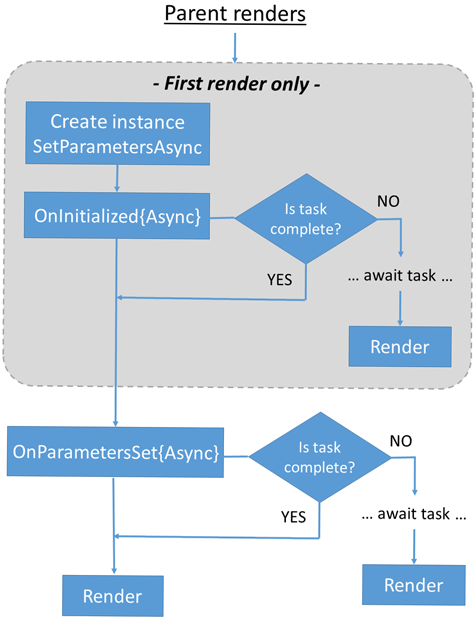
\includegraphics[width=80mm]{lifecycle1.png}}
\end{center}
\end{otherlanguage}


ככה שחשבתי על דרך לקרוא לסשן בזמן הגיוני, והוא לאחר שאדמין או משתמש מנסה לשלוח את הסיסמה שלו כדי לוודא את זהותו בפעם השנייה בכניסה לעמוד רגיש
\end{otherlanguage}
\end{document}